\documentclass[USenglish,twocolumn]{article}
\usepackage[utf8]{inputenc}
\usepackage[big,online]{dgruyter}
\usepackage{hypernat}
\setcitestyle{numbers,square,comma,sort&compress}

\begin{document}

%%%--------------------------------------------%%%
%%% Please do not alter the following 7 lines: %%%
%%%--------------------------------------------%%%
	\articletype{Proceedings}
  \journalname{Current~Directions~in~Biomedical~Engineering}
  \journalyear{2015}
  \journalvolume{1}
  \journalissue{???}
  \startpage{1}
  %\aop
  \DOI{10.1515/bmt-XXXX}
%%%--------------------------------------------%%%

\title{Insert your title here}
\runningtitle{Short title}
%\subtitle{Insert subtitle if needed}

\author*[1]{First Author}
\author[2]{Second Author}
\author[2]{Third Author} 
\runningauthor{F.~Author et al.}

\affil[1]{\protect\raggedright 
  Institution, address of first, e-mail: author\_one@rmi.ge}
\affil[2]{\protect\raggedright 
  Institution, address of second author and third author, e-mail: author\_two@rmi.ge, author\_three@rmi.ge}
	

\abstract{Hallo na Please insert your abstract here. Remember that online
systems rely heavily on the content of titles and abstracts to
identify articles in electronic bibliographic databases and search
engines. We ask you to take great care in preparing the abstract.}

\keywords{Please insert your keywords here, separated by commas.}

\maketitle

\section{Headline 1st level} 

Please insert your manuscript here. \textit{Please insert your manuscript here}. Please insert your manuscript here. Please insert your manuscript here. \textbf{Please insert your manuscript here}. Please insert your manuscript here. Please insert your manuscript here. Please insert your manuscript here. Please insert your manuscript here.

New paragraph: Please insert your manuscript here in \citep{2,3,4,5}. Please insert your manuscript here in \citep{1}. Please insert your manuscript here. Please insert your manuscript here. Please insert your manuscript here. Please insert your manuscript here.

\subsection{Headline 2nd level}
Please insert your manuscript here. Please insert your manuscript here. Please insert your manuscript here. Please insert your manuscript here. Please insert your manuscript here. Please insert your manuscript here. Please insert your manuscript here. Please insert your manuscript here. Please insert your manuscript here.

New paragraph: Please insert your manuscript here. Please insert your manuscript here. Please insert your manuscript here, see Table \ref{tab:Table1}. Please insert your manuscript here. Please insert your manuscript here. Please insert your manuscript here.

\begin{table}
\caption{Please insert your table caption here.}
\begin{tabular}{llr}
Table head 1 			& Table head 2 			& Table head 3 		\\ \midrule
Table content 1a 	& Table content 2a 	& Table content 3 \\
Table content 1b	& Table content 2b	& 0.1111 					\\
Table content 1c	& Table content 2c 	& 0.3333 					\\
\end{tabular}
\label{tab:Table1}
\end{table}

\subsubsection{Headline 3rd level}
Please insert your manuscript here. Please insert your manuscript here. Please insert your manuscript here. Please insert your manuscript here. Please insert your manuscript here. Please insert your manuscript here. Please insert your manuscript here. Please insert your manuscript here. Please insert your manuscript here.

New paragraph: Please insert your manuscript here. Please insert your manuscript here. Please insert your manuscript here. Please insert your manuscript here. Please insert your manuscript here. Please insert your manuscript here.
Please insert your manuscript here. Please insert your manuscript here. Please insert your manuscript here. Please insert your manuscript here. Please insert your manuscript here. Please insert your manuscript here. Please insert your manuscript here. Please insert your manuscript here. Please insert your manuscript here. Please insert your manuscript here. Please insert your manuscript here. Please insert your manuscript here. Please insert your manuscript here. Please insert your manuscript here. Please insert your manuscript here. Please insert your manuscript here.

\begin{itemize}
\item Item 1
\item Item 2
\end{itemize}

New paragraph: Please insert your manuscript here. Please insert your manuscript here. Please insert your manuscript here. Please insert your manuscript here. Please insert your manuscript here. Please insert your manuscript here.Please insert your manuscript here. Please insert your manuscript here. Please insert your manuscript here. Please insert your manuscript here. Please insert your manuscript here. Please insert your manuscript here. Please insert your manuscript here. Please insert your manuscript here. Please insert your manuscript here (see Figure \ref{img:Figure1}).

New paragraph: Please insert your manuscript here. Please insert your manuscript here. Please insert your manuscript here. Please insert your manuscript here. Please insert your manuscript here. Please insert your manuscript here.

%If possible, please provide figures in the grayscale or CMYK color mode rather than the RGB mode%
\begin{figure}
	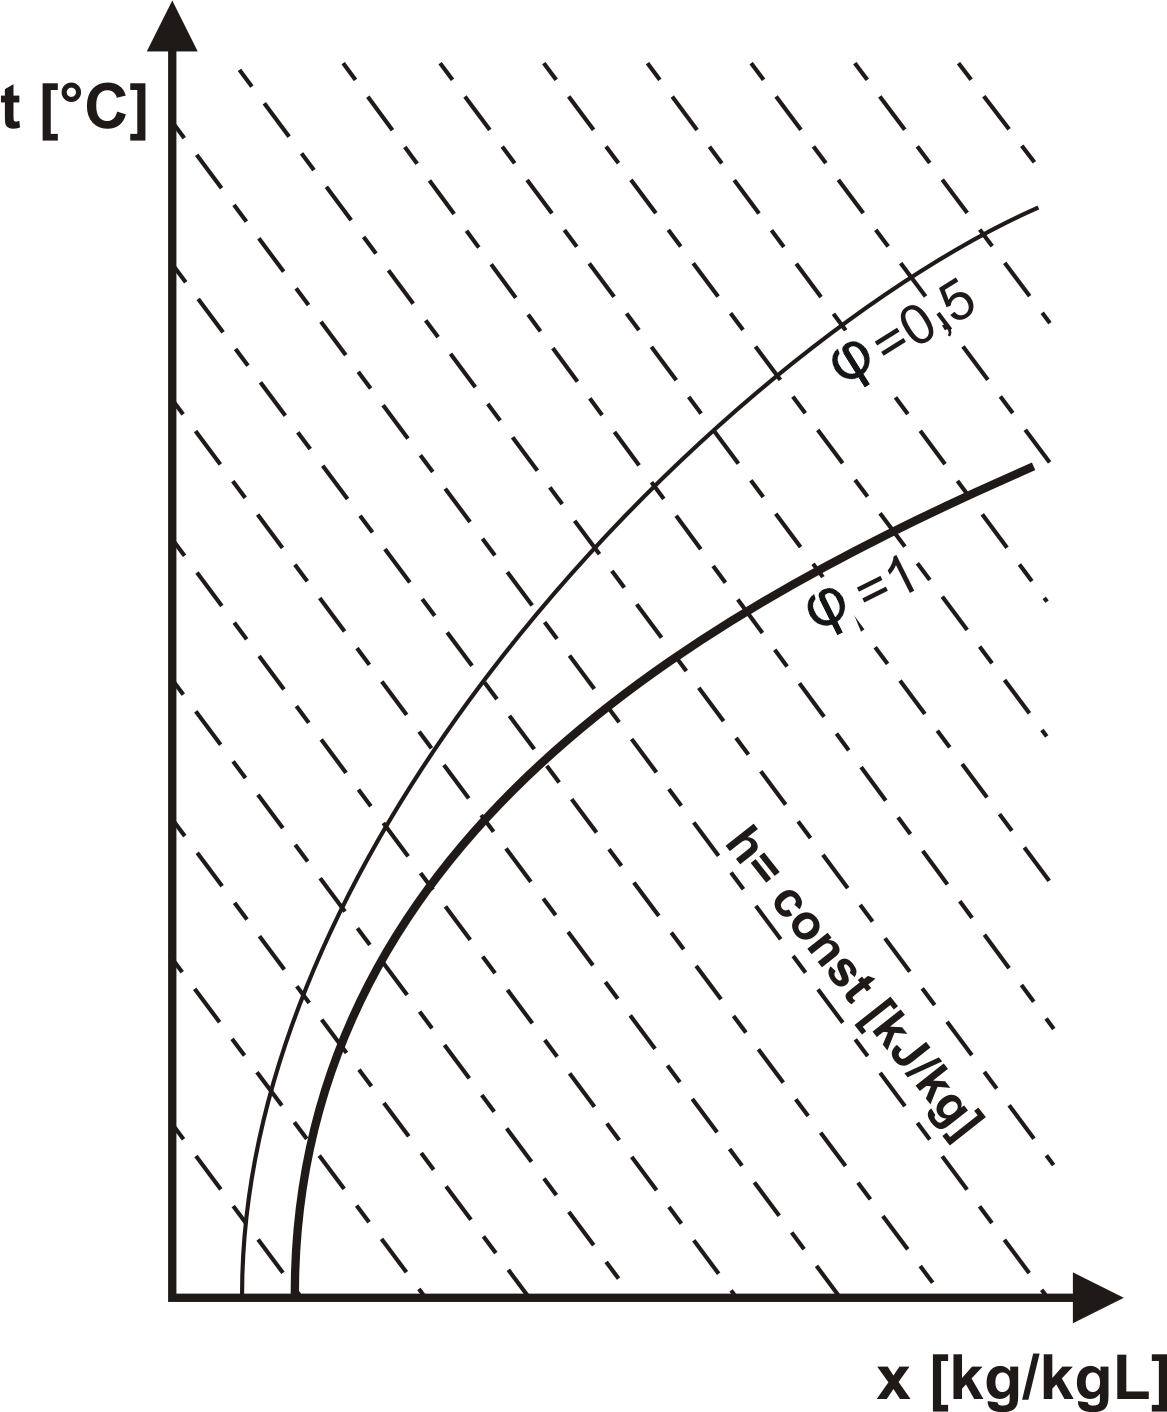
\includegraphics[width=\columnwidth]{graphics/figure1}
	\caption{Please insert your figure caption here.}
	\label{img:Figure1}
\end{figure}

\paragraph{Headline 4th level}
Please insert your manuscript here. Please insert your manuscript here. Please insert your manuscript here. Please insert your manuscript here. Please insert your manuscript here. Please insert your manuscript here. Please insert your manuscript here. Please insert your manuscript here. Please insert your manuscript here.

New paragraph: Please insert your manuscript here. Please insert your manuscript here. Please insert your manuscript here. Please insert your manuscript here. Please insert your manuscript here. 

In the subsequent discussion we can conveniently set
$$g=g_{0}, \quad a=a_{0}, \quad x=x_{0}+x_{1}2+x_{2}2^{2}+ \cdots +x_{n}2^{n}$$
$0 \leqslant x_{0}+x_{1}2+x_{2}2^{2}+ \cdots +x_{n}2^{n} \leqslant q-2,$
where $x_{i} \in \{0,1 \}$, for $0 \leqslant i \leqslant n$, and then
rewrite the relation (\ref{eq:1}) in the form

\begin{equation}\label{eq:1}
g_{0}^{x_{0}+x_{1}2+x_{2}2^{2}+ \cdots +x_{n}2^{n}}=a_{0} \mbox{ ,}
\end{equation}
Rising both parts of the last equation to the power $(q-1)/2$ and
taking into account that the following relation ...

\begin{enumerate}
\item Item 1
\item Item 2
\end{enumerate}

\begin{acknowledgement}
Please insert acknowledgments of the assistance of colleagues or similar notes of appreciation here.
\end{acknowledgement}

\def\acknowledgementname{Funding}
\begin{acknowledgement}
Please insert information concerning research grant support here
\end{acknowledgement}

%\bibliographystyle{...}
%\bibliography{...}

\begin{thebibliography}{9}
%---------------------------------------------------------------------------------------------------------------------%
% The Reference list at the end of the manuscript should be in alphanumerical order (see samples below).							%
%---------------------------------------------------------------------------------------------------------------------%

% Books
\bibitem{1}
Eisen HN. Immunology: an introduction to molecular and cellular
principles of the immune response. 5th ed. New York: Harper and
Row 1974.

% Institutional publications:
\bibitem{2}
Institute of Medicine (US). Looking at the future of the Medicaid
program. Washington: The Institute 1999.

% Chapters in books:
\bibitem{3}
Weinsten L, Swartz MN. Pathogenic properties of invading
microorganisms. In: Sodeman WA Jr, Sodeman WA, editors. Pathologic
physiology: mechanisms of disease. Philadelphia: WB Saunders 1974:
457--472.

% Articles in journals with up to 6 authors:
\bibitem{4}
Ge Q, Filip L, Bai A, Nguyen T, Eisen HN, Chen J. Inhibition
of influenza virus production in virus-infected mice by RNA interference.
Proc Natl Acad Sci USA 2004; 101: 8676--8681.

% Articles in journals with more than 6 authors:
\bibitem{5}
You CH, Lee KY, Chey WY, et al. Electrogastrographic study
of patients with unexplained nausea, bloating and vomiting. Gastroenterology 1980; 79: 311--314.

\end{thebibliography}
\end{document}
